\documentclass[12pt,brazil]{beamer}
\usepackage{graphicx}
\usepackage[brazil]{babel}
\selectlanguage{brazil}
\usepackage[utf8x]{inputenc}
\usepackage{subfig}
\usepackage{tikz}
\usepackage{blindtext}

%\usepackage[colorlinks]{hyperref}


% \title[teste]{TEste}

\begin{document}


{
\begin{frame}
    \begin{tikzpicture}[remember picture,overlay]
    \node[anchor=north west,yshift=-1.5pt,xshift=1pt]%
        at (current page.north west)
        {
\includegraphics[height=2cm]{figures/Brasao_da_UFBA.png}};
    \end{tikzpicture}
    \begin{tikzpicture}[remember picture,overlay]
    \node[anchor=north east,yshift=-1.5pt,xshift=1pt]%
        at (current page.north east)
        {
\includegraphics[height=2cm]{figures/brasao_escola_politecnica_0.jpg}};
    \end{tikzpicture}
    
    \centering{
    \textbf{UNIVERSIDADE FEDERAL DA BAHIA}
    
    \textbf{DEPARTAMENTO DE ENGENHARIA\\ELÉTRICA E DE COMPUTAÇÃO}
    }
    
    \hfill \break
    \hfill \break
    \hfill \break
    \centering{\textbf{Análise da latência de interrupção no Raspberry Pi com o kernel Linux e patches de tempo real}}
    
    \hfill \break
    \hfill \break
    \centering{Taian Fonseca Feitosa}
    
    \hfill \break
    \textbf{Orientador:} Dr. Paul Denis Etienne Regnier
    
    \hfill \break
    \centering{Salvador}
    
    \centering{05 de Dezembro de 2019}
    
    \hfill \break
    \hfill \break
    \hfill \break

\end{frame}
}





%pagina de contenido
\begin{frame}{Conteúdo}
\tableofcontents
\end{frame}


%La presentación en si
\section{Introdução}

\begin{frame}{Introdução}
\begin{itemize}
    \item Sistemas computacionais e requisitos temporais
    \item Sistemas operacionais de tempo real
    \item Raspberry Pi
\end{itemize}
\end{frame}

\section{Objetivos}

\begin{frame}{Objetivos}

Objetivo principal:
\begin{itemize}
    \item Verificar o determinismo do Raspberry Pi 3 Model B com o kernel padrão e com uma variação de tempo real.
\end{itemize}

Objetivos específicos:
\begin{itemize}
    \item Adaptar o INTSight para o Raspberry Pi;
    \item Realizar medições com o kernel padrão do Linux;
    \item Realizar medições com o kernel com patch Preempt-RT;
    \item Analisar o resultado obtido nas medições;
\end{itemize}
\end{frame}

\section{Linux}

\begin{frame}{Linux como sistema operacional de propósito geral}
\begin{itemize}
    \item Um dos sistemas operacionais mais utilizados em sistemas embarcados de prateleira.
    \item Sistema padrão do Raspberry Pi.
\end{itemize}
\end{frame}

\section{Interrupções}
\begin{frame}{Interrupções}
    \begin{itemize}
    \item O que é uma interrupção?
    \item Modelo de interrupção no Linux
\end{itemize}
\end{frame}

\begin{frame}{Mecanismos de tratamento de interrupção}
    \begin{itemize}
    \item Softirq
    \item Tasklet
    \item Workqueue
\end{itemize}
\end{frame}

\section{Sistemas Operacionais de Tempo Real}
\begin{frame}{Sistemas Operacionais de Tempo Real}
    \begin{itemize}
        \item Requisitos temporais
        \item Latências imprevisíveis
    \end{itemize}
    \begin{figure}[!htb]
        \centering
        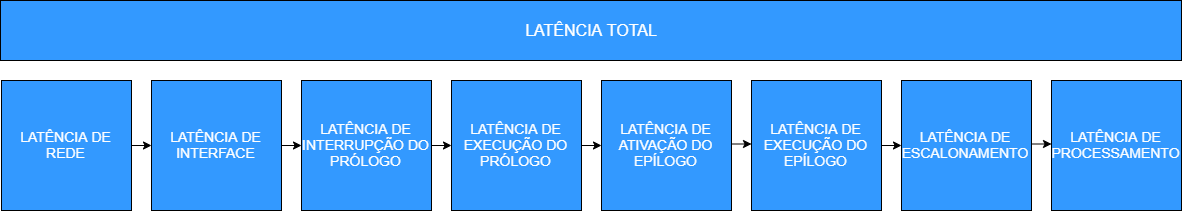
\includegraphics[width=\textwidth]{figures/latencias.png}
        \caption*{Latências envolvidas em uma instrução enviada pela rede}
    \end{figure}
\end{frame}

\section{Preempt-RT}
\begin{frame}{Preempt-RT}
    \begin{itemize}
        \item Patch que torna o kernel do Linux completamente preemptível.
    \end{itemize}
    
    Modos de preempção:
    \begin{figure}[!htb]
        \centering
        \subfloat[PREEMPT\_NONE]{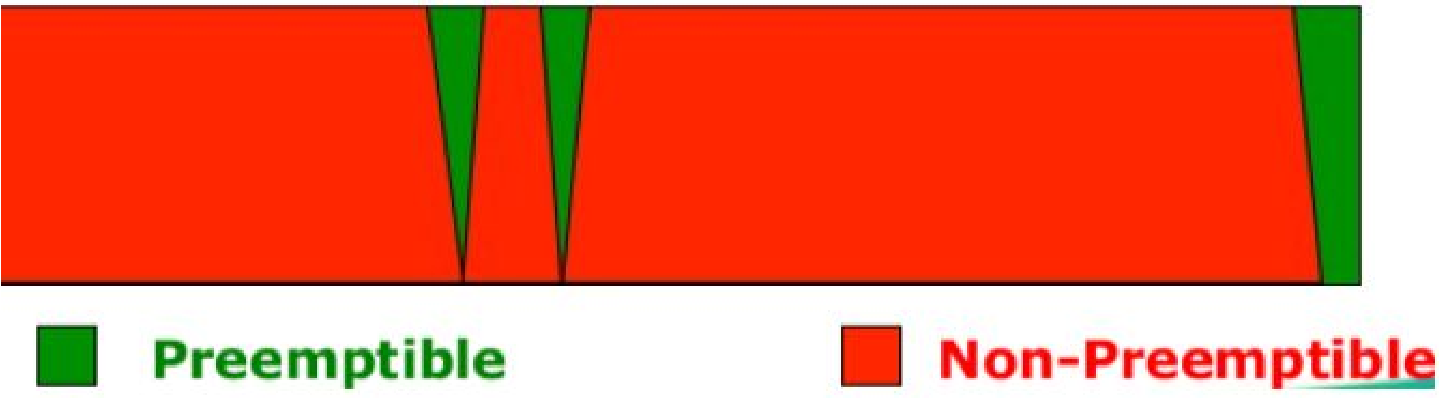
\includegraphics[width = .4\textwidth]{figures/PREEMPT_NONE.png}}%
        \subfloat[PREEMPT\_VOLUNTARY]{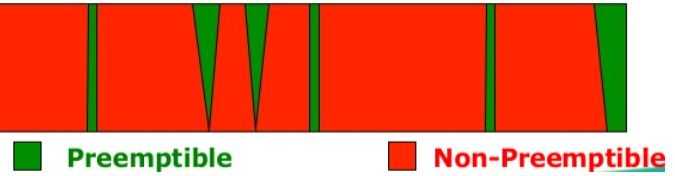
\includegraphics[width = .4\textwidth]{figures/PREEMPT_VOLUNTARY.png}}\\
        \subfloat[CONFIG\_PREEMPT]{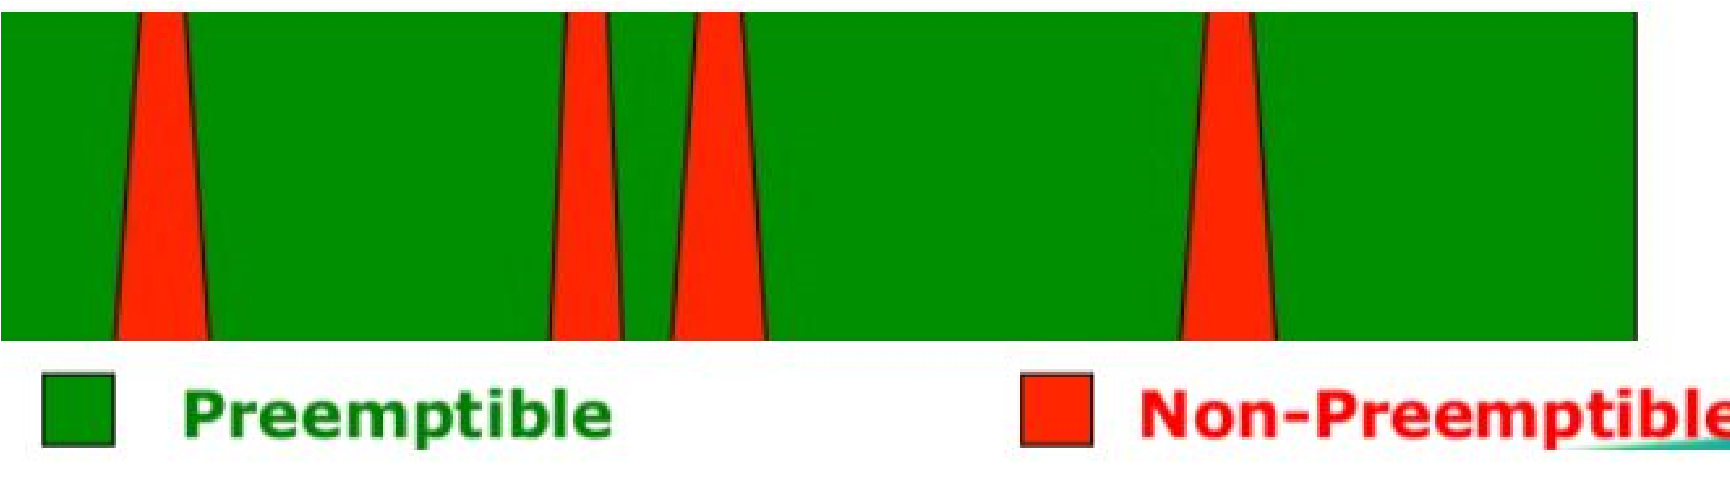
\includegraphics[width = .4\textwidth]{figures/CONFIG_PREEMPT.png}}%
        \subfloat[PREEMPT\_RT\_FULL]{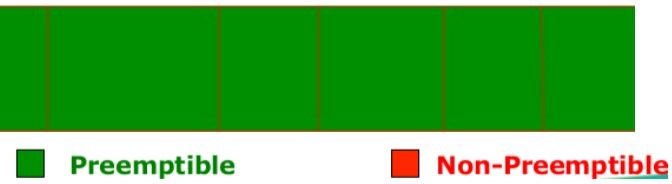
\includegraphics[width = .4\textwidth]{figures/PREEMPT_RT_FULL.png}} 
        \caption*{Configurações de preempção no kernel}
    \end{figure}

    % \begin{enumerate}[(a)]
    %   \item PREEMPT\_NONE: as preempções ocorrem apenas nas tarefas do usuário.
    %   \item PREEMPT\_VOLUNTARY: algumas partes do kernel tem pontos específicos que permitem a preempção.
    %   \item CONFIG\_PREEMPT: semelhantes ao PREEMPT\_VOLUNTARY mas com uma região de preempção maior.
    %   \item PREEMPT\_RT\_FULL: praticamente qualquer seção do kernel pode ser preemptada, exceto algumas partes extremamente críticas.
    % \end{enumerate}
\end{frame}

\section{Raspberry Pi}
\begin{frame}{Raspberry Pi}
    \begin{itemize}
        \item Computador completo em placa única
        \item Baixo consumo energético
        \item Linux como sistema operacional padrão
    \end{itemize}
    
    \begin{figure}[!htb]
        \centering
        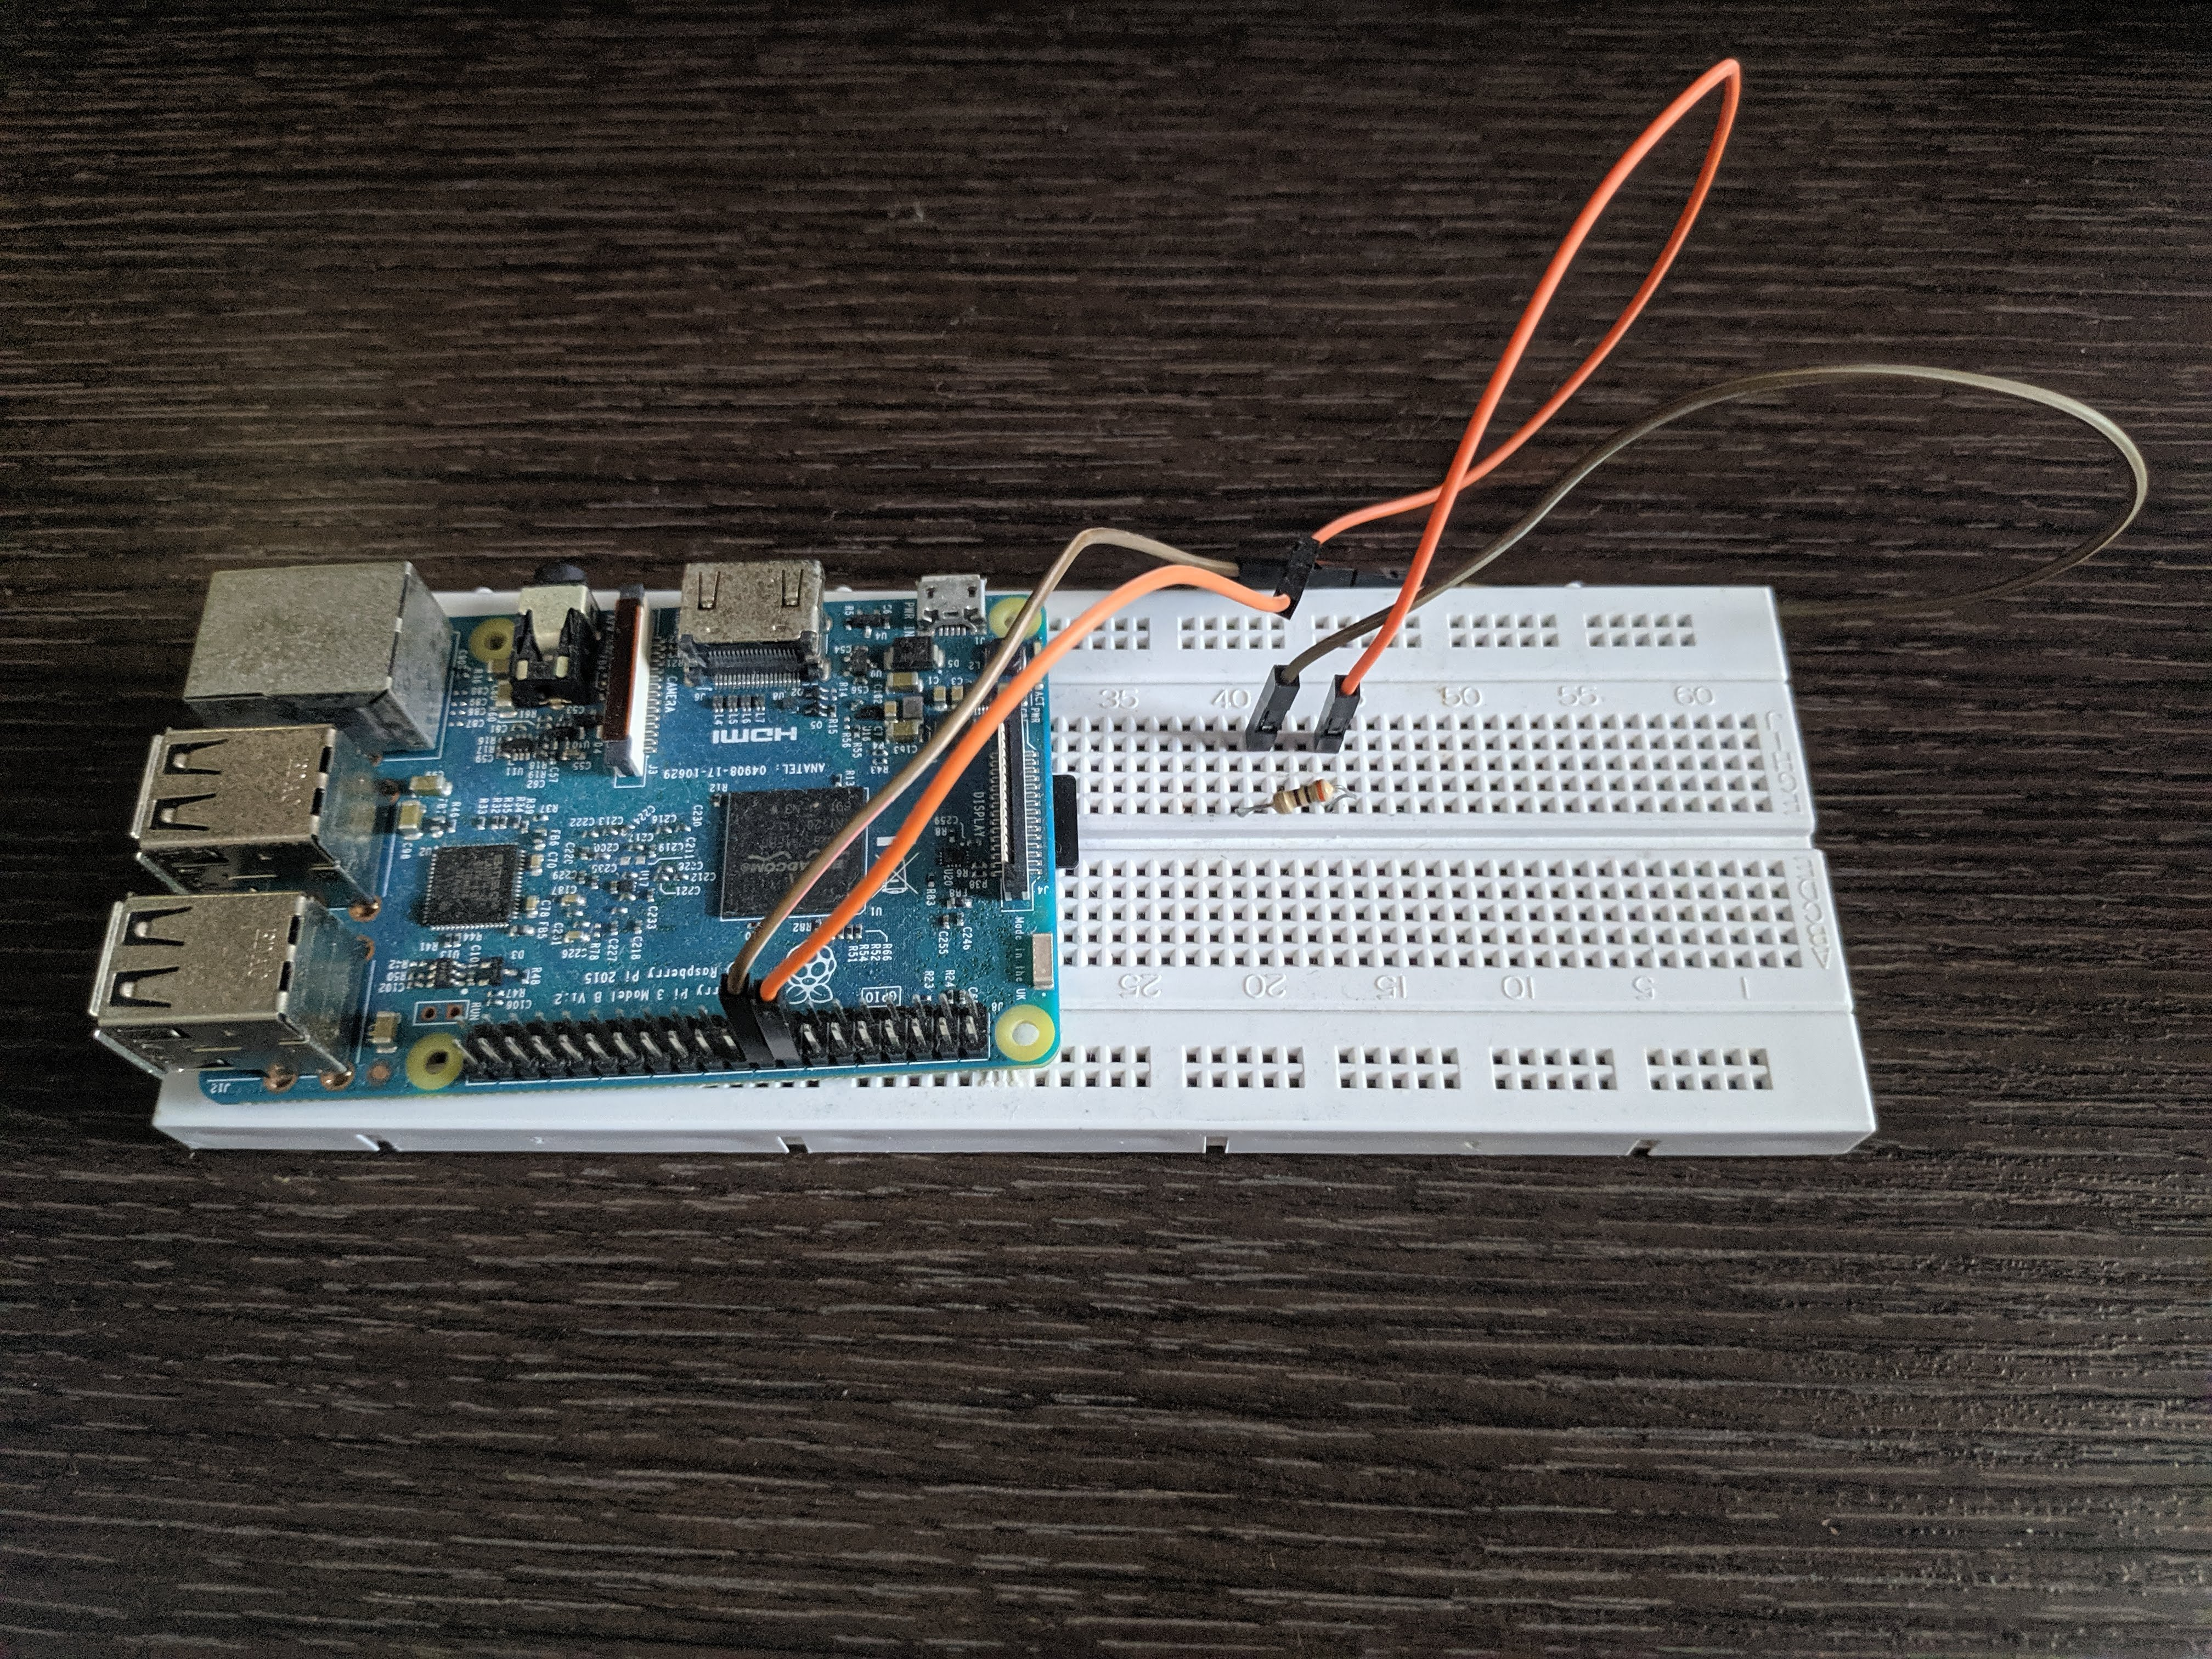
\includegraphics[width=.6\textwidth]{figures/raspberry-photo.jpg}
        \caption*{Foto do Raspberry Pi com a montagem feita para as medições}
        \label{foto:Raspberry Pi}
    \end{figure}
\end{frame}

\section{INTSight e INTSpect}
\begin{frame}{INTSight e INTSpect}
         INTSight:
        \begin{itemize}
            \item Módulo do kernel responsável pelas medições
            \item Alocado em tempo de compilação
            \item Precisão ao invés de flexibilidade
        \end{itemize}
         INTSpect:
        \begin{itemize}
            \item Módulo que dispara as medições no INTSight
        \end{itemize}
\end{frame}

\section{Medições}
\begin{frame}{Medições}
    Preparação do kernel durante a compilação:
    \begin{itemize}
        \item Suporte a temporizador de alta resolução;
        \item Controlador de frequência do processador configurado como \textit{Performance};
        \item Depurador do kernel desabilitado;
        \item Compactação de memória desabilitada;
        \item Alocação contígua de memória desabilitada;
    \end{itemize}
\end{frame}

\begin{frame}{Medições}
    Grupos de testes:
    \begin{itemize}
        \item Versão do kernel
        \begin{itemize}
            \item Padrão (R)
            \item Prempt-RT (P)
        \end{itemize}
        \item Mecanismo de interrupção
        \begin{itemize}
            \item Softirq (S)
            \item Tasklet (T)
            \item Workqueue (W)
        \end{itemize}
        \item Carga no processador
        \begin{itemize}
            \item 0 thread (0)
            \item 1 thread (1)
            \item 256 threads (M)
        \end{itemize}
    \end{itemize}
    Total de 18 combinações possíveis.
\end{frame}

\begin{frame}{Medições}
    Padrão de siglas:
    \begin{itemize}
        \item RS0: Teste com o kernel padrão, mecanismo Softirq e 0 threads de carga no processador.
        \item PWM: Teste com o Preempt-RT, mecanismo Workqueue e 256 threads de carga no processador.
    \end{itemize}
\end{frame}

\begin{frame}{Medições}
Principais dados das medições com o kernel padrão, em nanossegundos.
    \begin{figure}[!htb]
        \centering
        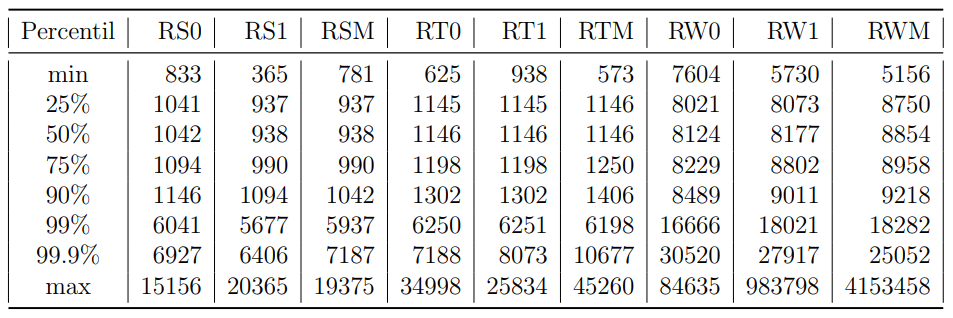
\includegraphics[width=\textwidth]{figures/tabela_r.png}
        \label{table:rasp}
    \end{figure}

\end{frame}

\begin{frame}{Medições}
Principais dados das medições com o Preempt-RT, em nanossegundos.
    \begin{figure}[!htb]
        \centering
        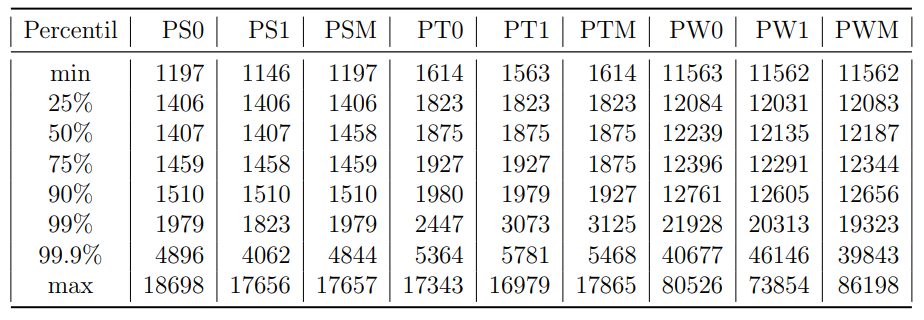
\includegraphics[width=\textwidth]{figures/tabela_p.png}
        \label{table:rasp}
    \end{figure}

\end{frame}

\begin{frame}{Medições - Softirq}
    
    \begin{figure}[!htb]
        \centering
        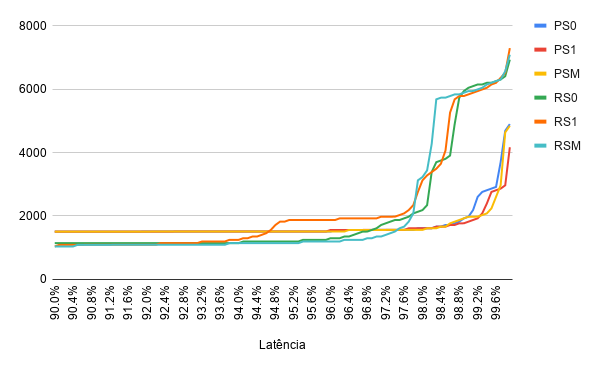
\includegraphics[width=\textwidth]{figures/softirq.png}
        \caption*{Latência com Softirq em nanossegundos}
        \label{grafico:softirq}
    \end{figure}

\end{frame}

\begin{frame}{Medições - Softirq}
    
    \begin{figure}[!htb]
        \centering
        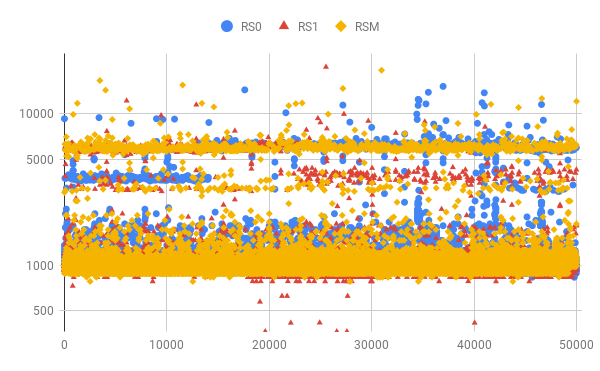
\includegraphics[width=\textwidth]{figures/rs-scatter.png}
        \caption*{Latência da sequência de testes com Softirq no kernel padrão}
        \label{grafico:r-softirq}
    \end{figure}

\end{frame}

\begin{frame}{Medições - Softirq}
    
    \begin{figure}[!htb]
        \centering
        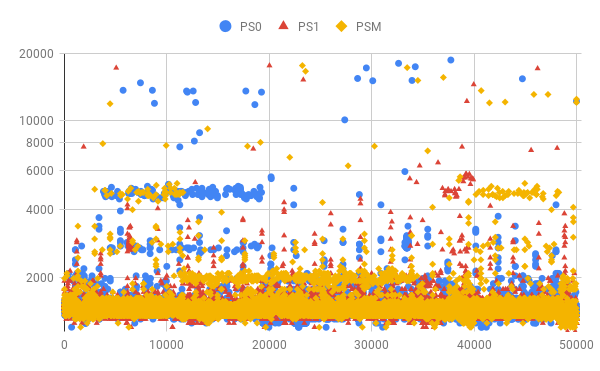
\includegraphics[width=\textwidth]{figures/ps-scatter.png}
        \caption*{Latência da sequência de testes com Softirq no Preempt-RT}
        \label{grafico:r-softirq}
    \end{figure}

\end{frame}

\begin{frame}{Medições - Tasklet}
    
    \begin{figure}[!htb]
        \centering
        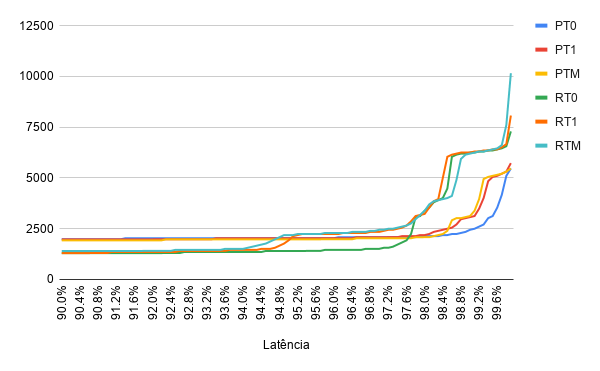
\includegraphics[width=\textwidth]{figures/tasklet.png}
        \caption*{Latência com Tasklet em nanossegundos}
        \label{grafico:softirq}
    \end{figure}

\end{frame}

\begin{frame}{Medições - Tasklet}
    
    \begin{figure}[!htb]
        \centering
        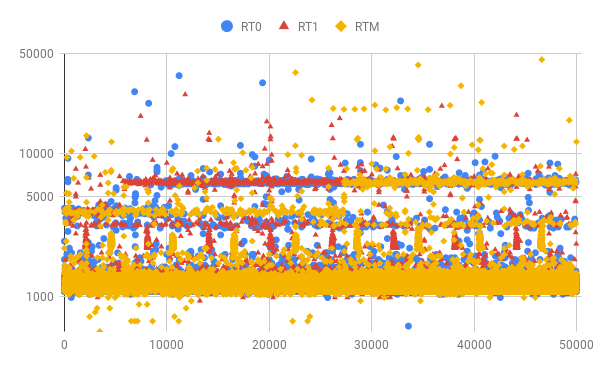
\includegraphics[width=\textwidth]{figures/rt-scatter.png}
        \caption*{Latência da sequência de testes com Tasklet no kernel padrão}
        \label{grafico:r-softirq}
    \end{figure}

\end{frame}

\begin{frame}{Medições - Tasklet}
    
    \begin{figure}[!htb]
        \centering
        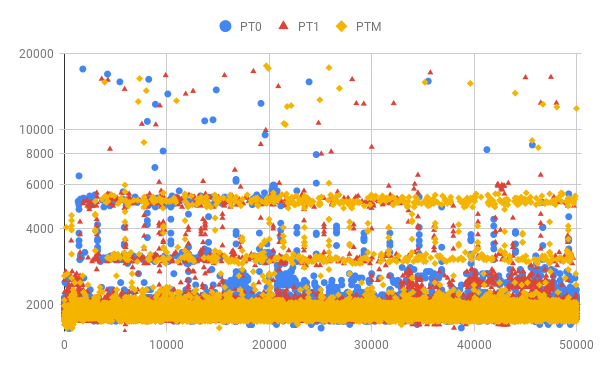
\includegraphics[width=\textwidth]{figures/pt-scatter.png}
        \caption*{Latência da sequência de testes com Tasklet no Preempt-RT}
        \label{grafico:r-softirq}
    \end{figure}

\end{frame}

\begin{frame}{Medições - Workqueue}
    
    \begin{figure}[!htb]
        \centering
        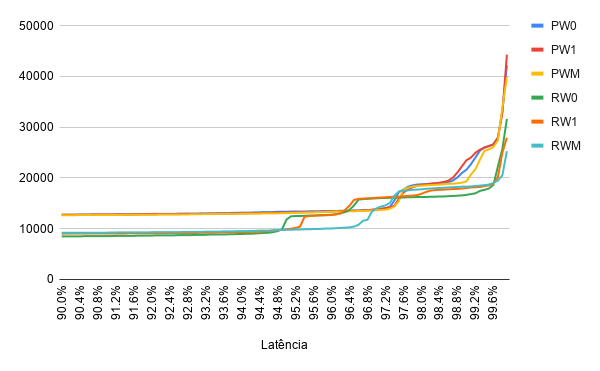
\includegraphics[width=\textwidth]{figures/workqueue.png}
        \caption*{Latência com Workqueue em nanossegundos}
        \label{grafico:softirq}
    \end{figure}

\end{frame}

\begin{frame}{Medições - Workqueue}
    
    \begin{figure}[!htb]
        \centering
        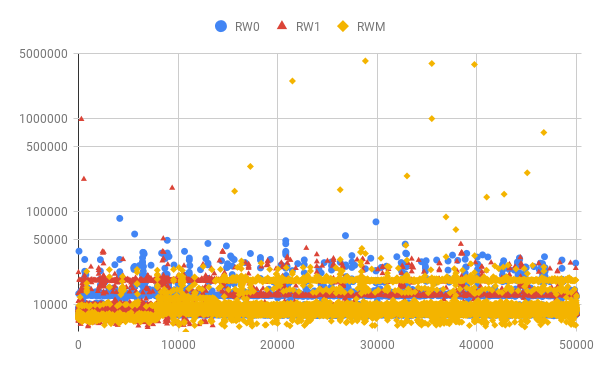
\includegraphics[width=\textwidth]{figures/rw-scatter.png}
        \caption*{Latência da sequência de testes com Workqueue no kernel padrão}
        \label{grafico:r-softirq}
    \end{figure}

\end{frame}

\begin{frame}{Medições - Workqueue}
    
    \begin{figure}[!htb]
        \centering
        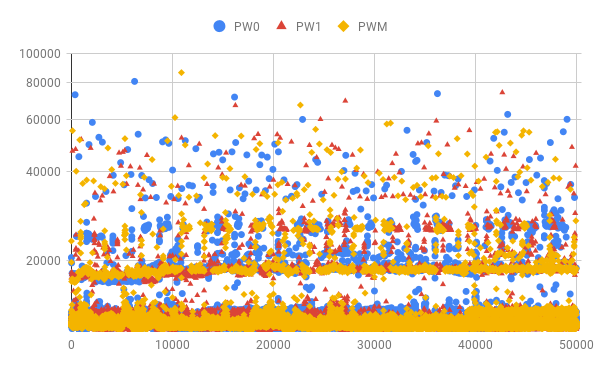
\includegraphics[width=\textwidth]{figures/pw-scatter.png}
        \caption*{Latência da sequência de testes com Workqueue no Preempt-RT}
        \label{grafico:r-softirq}
    \end{figure}

\end{frame}

\begin{frame}{Medições - Impressões}
    Softirq:
    \begin{itemize}
        \item Não varia significativamente com a carga;
        \item Diferença pouco significativa entre a versão padrão e a versão de tempo real para o pior caso;
        \item Versão padrão possui caso médio melhor;
        \item Implementação exige recompilação do kernel, pouco flexível;
    \end{itemize}
\end{frame}

\begin{frame}{Medições - Impressões}
    Tasklet:
    \begin{itemize}
        \item Não varia significativamente com a carga;
        \item Diferença significativa entre a versão padrão e a versão de tempo real para o pior caso;
        \item Versão padrão possui caso médio melhor e o pior caso aparenta ter um limite;
        \item Implementação como módulo de kernel, mais flexível que o Softirq e não há limite na quantidade de Tasklets que podem ser implementados;
    \end{itemize}
\end{frame}

\begin{frame}{Medições - Impressões}
    Workqueue:
    \begin{itemize}
        \item Na versão padrão, é sensível a carga no processador;
        \item No Preempt-RT, a carga não influencia a latência significativamente;
        \item Diferença muito grande entre a versão padrão e a versão de tempo real para o pior caso quando o processador está carregado;
        \item Implementação mais flexível, porém com maior custo;
    \end{itemize}
\end{frame}

\section{Conclusão}

\begin{frame}{Conclusão}
    Foi apresentado:
    \begin{itemize}
        \item Mecanismos de interrupção;
        \item Patche de tempo real - Preempt-RT;
        \item Medição de latência no Raspberry Pi;
    \end{itemize}
\end{frame}

\begin{frame}{Conclusão}
    Futuro:
    \begin{itemize}
        \item Adaptar o Xenomai;
        \item Comparar os resultados do Xenomai com o Preempt-RT;
    \end{itemize}
\end{frame}

\section{Referências Bibliográficas}

\begin{frame}{REFERÊNCIAS BIBLIOGRÁFICAS}

\begin{itemize}
    \item BURNS, A.; WELLINGS, A. \textit{Real-Time Systems and Programming Languages.} [S.l.: s.n.], 2001. ISBN 0-471-22855-9.
    \item CARTWRIGHT, J. \textit{Embedded Linux Conference in Portland}. 2018.
    \item CESATI, M.; BOVET, D. P. \textit{Understanding the Linux Kernel.} [S.l.]: O’Reilly Media, Inc., 2005. ISBN 0596005652.
    \item CORBET, J.; RUBINI, A.; KROAH-HARTMAN, G. \textit{Linux Device Drivers.} [S.l.]: O’Reilly Media, Inc., 2009. ISBN 0-596-00590-3.
    \item GERHORST, L. \textit{Analysis of Interrupt Handling Overhead in the Linux Kernel.} TCC — Friedrich-Alexander-Universit ̈at Erlangen-Nürnberg (FAU), 2018.
\end{itemize}

\end{frame}

\begin{frame}{REFERÊNCIAS BIBLIOGRÁFICAS}

\begin{itemize}
    \item HUANG, J.; CHUNG-FAN. \textit{Effectively Measure and Reduce Kernel Latencies for Real-time Constraints.} 2017.
    \item JOHANSSON, G. \textit{Real-Time Linux Testbench on Raspberry Pi 3 using Xenomai.} Degree Project — KTH ROYAL INSTITUTE OF TECHNOLOGY, 2018.
    \item Linux Foundation. \textit{Intro to Real-Time Linux for Embedded Developers.} 2013.
    \item LIU, J. W. S. \textit{Real-Time Systems.} [S.l.]: Prentice-Hall, 2000. ISBN 978-0130996510.
    \item MCKENNEY, P. A \textit{realtime preemption overview.} 2015.
    \item MOLNAR, I. \textit{CONFIG PREEMPT RT Patch.} 2016. 
    \item PRATT, S. G.; HEGER, D. A. \textit{Workload Dependent Performance Evaluation of the Linux 2.6 I/O Schedulers.} 2004.
\end{itemize}
    
\end{frame}

\begin{frame}{REFERÊNCIAS BIBLIOGRÁFICAS}

\begin{itemize}
    \item PUHLMANN, H. F. W. \textit{Sistemas Operacionais de Tempo Real - Introdução.} 2014.
    \item REGNIER, P.; LIMA, G.; BARRETO, L. \textit{Avaliação do determinismo temporal no tratamento de interrupções em plataformas de tempo real Linux. WSO – Workshop de Sistemas Operacionais,} 2008.
    \item ROTHBERG, V. \textit{Interrupt Handling in Linux.} [S.l.], 2015.
    \item SOLOMON, D. A.; RUSSINOVICH, M. \textit{Inside Microsoft Windows.} [S.l.]: David Solomon Expert Seminars, Inc., 2000. ISBN 3-86063-630-8.
    \item WILCOX, M. \textit{I’ll do it later: Softirqs, tasklets, bottom halves, task queues, work queues and timers. Proceedings of the 3rd linux.conf.au Conference.}, 2003.
\end{itemize}

\end{frame}
{
\begin{frame}
    \begin{tikzpicture}[remember picture,overlay]
    \node[anchor=north west,yshift=-1.5pt,xshift=1pt]%
        at (current page.north west)
        {
\includegraphics[height=2cm]{figures/Brasao_da_UFBA.png}};
    \end{tikzpicture}
    \begin{tikzpicture}[remember picture,overlay]
    \node[anchor=north east,yshift=-1.5pt,xshift=1pt]%
        at (current page.north east)
        {
\includegraphics[height=2cm]{figures/brasao_escola_politecnica_0.jpg}};
    \end{tikzpicture}

    \begin{minipage}[t]{\linewidth} % ajustar el parametro 0.8 para visualizar mejor el título
% {\textcolor{}{Análise da latência de interrupção no Raspberry Pi com o kernel Linux e patches de tempo real}} %opciones \Huge \HUGE \Large \Large
\\
\\
%-------------------------------------------
\centering{ \textcolor{}{Taian Fonseca Feitosa}} %opciones \Huge \HUGE \Large \Large \small \tiny
\\
\centering{ \textcolor{}{taianmeca@gmail.com}}  
%--------------------------------------------
\\
\\
%-------------------------------------------
% { \textcolor{white}{Nombre del autor 2}} %opciones \Huge \HUGE \Large \Large \small \tiny
\\
% { \textcolor{white}{correo2@correo.com}}  
%--------------------------------------------
\\

%-------------------------------------------
% { \textcolor{white}{Nombre del autor 3}} %opciones \Huge \HUGE \Large \Large \small \tiny
\\
% { \textcolor{white}{correo3@correo.com}}  
%--------------------------------------------

\end{minipage}
\end{frame}
}

{
\begin{frame}{}
    \centering
    \HUGE \textbf{OBRIGADO!}
\end{frame}
}
\end{document}